\documentclass{standalone}
\usepackage{fkmath, tikz}
\usetikzlibrary{tikzmark}


% \usetikzlibrary{}
\begin{document}
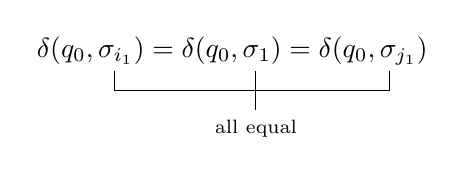
\begin{tikzpicture}
  \node (eq) at (0,0) {$\delta(q_0, \tikzmarknode{si1}{\sigma_{i_1}})
    = \delta(q_0, \tikzmarknode{s1}{\sigma_1}) = \delta(q_0,
    \tikzmarknode{sj1}{\sigma_{j_1}})$};
  \begin{scope}
    \coordinate (si1) at (-1.5, -.25);
    \coordinate (s1)  at (0.3,  -.25);
    \coordinate (sj1)  at (2,  -.25);

    \draw (si1) -- ++(0, -.25) node[coordinate, at end] (a) {};
    \draw (s1) -- ++(0, -.25) node[coordinate, at end] (b) {};
    \draw (sj1) -- ++(0, -.25) node[coordinate, at end] (c) {};
    \draw (a) -- (b) -- (c);
    \draw (b) -- ++(0,-.25) node[at end, below] {\scriptsize all equal};
  \end{scope}
\end{tikzpicture}

% $\displaystyle

% $
% \begin{tikzpicture}[overlay, remember picture]

% \end{tikzpicture}
\end{document}
